% !TEX options=--shell-escape
\documentclass[a4paper,11pt]{article}
\usepackage[english]{babel}
\usepackage{fancyhdr} 
\usepackage{times} 
\usepackage{amsmath}
\usepackage{amsfonts}
\usepackage{colortbl}
\usepackage{color}
\usepackage{rotating}
\usepackage{xspace}
\usepackage{epsfig}
\usepackage{subfigure} 
\usepackage[mark]{gitinfo2}
\usepackage{lmodern}
\usepackage[utf8x]{inputenc}
\usepackage[LGR,T1]{fontenc}
\usepackage[normalem]{ulem} 
\usepackage{pgfplots}
\usetikzlibrary{shadows}
%\usepackage{fullpage}
\usepackage[a4paper, lmargin = {2.5cm}, rmargin={2.5cm}, tmargin={3cm}, bmargin={2.5cm}, includefoot]{geometry}
\usepackage[pagebackref=true,breaklinks=true,colorlinks,linkcolor=blue,bookmarks=true]{hyperref}
\usepackage{lscape}
\usepackage{sectsty}
\usepackage{import}
\usepackage{minted}
\usepackage[autostyle=true]{csquotes}
\usepackage[super]{nth}
\usepackage{relsize}
\usepackage{framed}
\usepackage[colorinlistoftodos]{todonotes}

\setlength{\headheight}{15pt}

\allsectionsfont{\normalfont \bfseries \sffamily \color{mycolor}}
\definecolor{mycolor}{rgb}{0.09,0.09,0.5}
% \definecolor{mycolor}{rgb}{0.25,0.25,0.25}
\definecolor{lightgrey}{rgb}{0.8,0.8,0.8}
\definecolor{bg}{rgb}{0.90,0.90,0.90}
\definecolor{shadecolor}{rgb}{0.8,0.8,0.8}
\definecolor{anscol}{rgb}{0.9,0.3,0.3}
% \definecolor{TFFrameColor}{rgb}{0.8,0.8,0.8}
\definecolor{TFFrameColor}{rgb}{0.8,0.8,1.0}
\definecolor{TFTitleColor}{rgb}{0.09,0.09,0.5}

\makeatletter
\DeclareRobustCommand\onedot{\futurelet\@let@token\@onedot}
\def\@onedot{\ifx\@let@token.\else.\null\fi\xspace}
\DeclareRobustCommand\nodot{\futurelet\@let@token\@nodot}
\def\@nodot{\ifx\@let@token.\else~\null\fi\xspace}

\def\eg{\emph{e.g}\onedot} \def\Eg{\emph{E.g}\onedot}
\def\ie{\emph{i.e}\onedot} \def\Ie{\emph{I.e}\onedot}
\def\cf{\emph{c.f}\onedot} \def\Cf{\emph{C.f}\onedot}
\def\etc{\emph{etc}\onedot} \def\vs{\emph{vs}\onedot}
\def\na{\emph{n.a}\onedot} \def\NA{\emph{N.A}\onedot}
\def\wrt{w.r.t\onedot} 
\def\dof{d.o.f\onedot}
\def\etal{\emph{et al}\onedot}
\makeatother

%put a wide hat over the argumetn
\newcommand{\lift}[1]{\ensuremath{\widehat{#1}}}

%put a wide hat over the argumetn
%\newcommand{\lifto}[1]{\ensuremath{\check{#1}}}
\newcommand{\lifto}[1]{\ensuremath{\overset{_{_{\circ}}}{#1}}}


% stack vector
\newcommand{\stackv}[1]{\ensuremath{\vet{v}\left( {#1} \right)}}
\newcommand{\ustackv}[1]{\ensuremath{\inv{\vet{v}}\left( {#1} \right)}}

% symmetric stack vector
\newcommand{\stackvs}[1]{\ensuremath{\vet{v}_{\textit{sym}}\left( {#1} \right)}}

% Matrix Lifting: put a wide hat over the argument intended to be a matrix
\newcommand{\mlift}[1]{\ensuremath{\lift{\mat{#1}}}}
\newcommand{\mlifto}[1]{\ensuremath{\lifto{\mat{#1}}}}

% Vector Lifting: put a wide hat over the argument intended to be a matrix
\newcommand{\vlift}[1]{\ensuremath{\lift{\vet{#1}}}}
\newcommand{\vlifto}[1]{\ensuremath{\lifto{\vet{#1}}}}

\newcommand{\bmat}[1]{\ensuremath{\begin{bmatrix} #1 \end{bmatrix}}}
% Vector: print the argument as a vector
\newcommand{\vet}[1]{\ensuremath{\mathbf{#1}}}

% Matrix: print the argument as a matrix
\newcommand{\mat}[1]{\ensuremath{\,\mathtt{\uppercase{#1}}\,}}

% Inverse: print a -1 on the top right of the argument 
\newcommand{\inv}[1]{\ensuremath{{#1}^{\text{-}1}}}

% Inverse: print a -1 on the top right of the argument 
\newcommand{\minv}[1]{\ensuremath{\mat{{#1}}^{\text{-}1}}}

% Transpose: print a T on the top right of the argument 
\newcommand{\tra}[1]{\ensuremath{{#1}^{\top}}\,}

% Transpose Matrix: print a T on the top right of the argument intended to be a matrix 
\newcommand{\mtra}[1]{\ensuremath{\tra{\mat{#1}}}}

% Transpose Vector: print a T on the top right of the argument intended to be a vector
\newcommand{\vtra}[1]{\ensuremath{\tra{\vet{#1}}}}

% minus transpose:  print a -T on the top right of the argument
\newcommand{\ment}[1]{\ensuremath{{#1}^{\text{--}\mathsf{T}}}}

% Cross Matrix:  print the argument in the cross matrix notation
\newcommand{\crmat}[1]{\ensuremath{\left[{#1}\right]_{\times}}}

\newcommand{\norm}[1]{\ensuremath{\left|\left|{#1}\right|\right|}}

\DeclareMathOperator{\diag}{diag}
\DeclareMathOperator{\rank}{rank}
  
 

\newcommand{\executeiffilenewer}[3]{%
\ifnum\pdfstrcmp{\pdffilemoddate{#1}}%
{\pdffilemoddate{#2}}>0%
{\immediate\write18{#3}}\fi%
}
\newcommand{\includesvg}[1]{%
\executeiffilenewer{#1.svg}{#1.pdf}%
{inkscape -z -D --file=#1.svg %
--export-pdf=#1.pdf --export-latex}%
\import{}{#1.pdf_tex}%
}

\newcommand{\hilight}[1]{\colorbox{bg}{#1}}
\newcommand{\coden}[1]{\texttt{#1}}
\newcommand{\code}[1]{\hilight{\texttt{#1}}}
\newcommand{\hired}[1]{\colorbox{anscol}{#1}}


\newcommand{\brand}[1]{\textsf{#1}\xspace}
\newcommand{\opengl}{\brand{OpenGL}}
\newcommand{\OpenGL}{\opengl}
\newcommand{\GLUT}{\brand{GLUT}}
\newcommand{\glut}{\GLUT}
\newcommand{\obj}{\brand{OBJ}}
\newcount\nextyear
\nextyear=\year
\advance\nextyear by 1
\newcount\prevyear
\prevyear=\year
\advance\prevyear by -1
\newcommand{\ayear}{\the\year-\the\nextyear}
\newcommand{\ayearSecond}{\the\prevyear-\the\year}

\newcommand{\todocode}[1]{\todo[color=green!40]{#1}}

% \newcommand{\answer}[1]{{\color{anscol} \textbf{#1}}}
 \newcommand{\answer}[1]{}

\newcommand*\keystroke[1]{%
  \tikz[baseline=(key.base)]
	\node[%
	  draw,
	  fill=white,
	  drop shadow={shadow xshift=0.25ex,shadow yshift=-0.25ex,fill=black,opacity=0.75},
	  rectangle,
	  rounded corners=2pt,
	  minimum size=5mm,
	  inner sep=1pt,
	  line width=0.5pt,
	  font=\scriptsize\sffamily
	](key) {#1\strut}
  ;
}

\newenvironment{stack}%
{\begin{center}
\begin{tikzpicture}[node distance=0mm,
terminal/.style={rectangle, minimum height=6mm,minimum width=32mm,rounded corners=3mm,very thick,draw=blue!50,top color=white,bottom color=blue!20,font=\ttfamily},
nonterminal/.style={rectangle,minimum width=3mm,top color=white,font=\ttfamily}]}
{\end{tikzpicture} 
\end{center} }


\newminted{bash}{bgcolor=bg}
\newminted{cpp}{bgcolor=bg, linenos=true}

%reference to Figure with mbox
% \newcommand{\fig}[1]{\mbox{Figure \ref{#1}}}
\newcommand{\fig}[1]{\hyperref[#1]{\mbox{Figure \ref*{#1}}}\xspace}

%reference to Table with mbox
\newcommand{\tab}[1]{\mbox{Table \ref{#1}}}

%reference to Section with mbox 
% \newcommand{\sect}[1]{\mbox{\S \ref{#1}}}
\newcommand{\sect}[1]{\hyperref[#1]{\mbox{Section \ref*{#1}}}\xspace}

\newcommand{\course}{Modélisation et rendu}

\title{\sf\bfseries TP5 - Working with meshes \\ {\small Visualizing more complex 3D objects}}
\author{\course, \ayearSecond\\ \nth{2} year, Multimedia track}
% \date{December \nth{4}, \the\year}
\date{Session 5\\~\\{\small Version: \gitReln{} \\\vskip -2mm {\tiny (\gitBranch\,@\,\gitAbbrevHash{} \gitAuthorDate)}}}
\pagestyle{fancyplain}
\fancyhead[R]{\sf \course, \ayearSecond}
% \fancyhead[L]{\sf INPT-ENSEEIHT}
\fancyhead[L]{
\includegraphics[height=5mm]{inp-enseeiht.jpg}}


\setcounter{secnumdepth}{5}
\setcounter{tocdepth}{5}


\begin{document}

\maketitle
\textsf{\tableofcontents}

\section{Objective}
In this last TP we will see one more aspect of the \opengl modeling by building a simple viewer of 3D meshes defined in a standard format, the \obj format. This will allow us to introduce a more efficient way to draw the geometric primitives \opengl and to implement a subdivision algorithm.


% \subsection{Assignments}
% These TPs are not graded, anyway you are invited to try to work in \uline{group of two} ({\href{https://en.wikipedia.org/wiki/Pair_programming}{pair programming}) and, in order to get a feedback or solve some issues with the code, send the code in a file named \code{surname1-surname2.cpp} to the mail address of your tutor\\ (\coden{\{simone.gasparini\}@enseeiht.fr}) with \coden{[VSI-TP5-\the\year]} as subject.

% \subsection{\opengl references}

% {\smaller Some useful resources about \opengl in general and the topics we will cover in this TP:
% \begin{itemize}
% \item Chapter 2 of the \emph{OpenGL Programming Guide}, covers the vertex arrays. You can find the on-line version at this address \url{http://www.glprogramming.com/red/chapter05.html}


% \item \emph{OpenGL et GLUT: Une Introduction}, by Edmond Boyer (INRIA Grenoble-Rhône--Alpes), in French. \url{http://www.ann.jussieu.fr/hecht/ftp/DEA/OpenGL.pdf}
% \item \opengl function documentation  \url{http://www.opengl.org/sdk/docs/man4/}
% \item \glut function documentation  \url{http://www.opengl.org/resources/libraries/glut/spec3/spec3.html}
% \item Google it!\ldots The easiest way to found the documentation of a function (or help) is to google the name of the function.
% \end{itemize}
% }



\section{Efficient drawing in \opengl: the vertex arrays}
\label{sec:arrays}


So far we have drawn 3D objects calling the function \coden{glVertexf()} for each single vertex: in the case of the icosahedron, \eg, we drew each triangle using 3 calls to \coden{glVertexf()}. In general, each time we call a function we also introduce a small overhead in the computation, hence when dealing with meshes with many triangles, a huge overhead is introduced that affect the performances of the program.

\OpenGL has another way to deal with large meshes, the vertex arrays. These routines allow you to specify a lot of vertex-related data with just a few arrays and to access that data with equally few function calls: \eg all the vertices of the mesh can be collected into a single array and draw with a single instruction. In order to use the vertex arrays there are 3 main steps to follow:

\begin{enumerate}
	\item Activate and enable the arrays, each storing a different type of data: vertex coordinates, RGBA colors, color indices, surface normals, vertex indices, texture coordinates. \opengl provides the function \coden{glEnableClientState()} which activates the type of array (vertices, normals, \etc):\\

{\smaller
\begin{cppcode}
// Specifies the array to enable. Symbolic constants GL_VERTEX_ARRAY, GL_COLOR_ARRAY, 
//GL_INDEX_ARRAY, GL_NORMAL_ARRAY, GL_TEXTURE_COORD_ARRAY, and GL_EDGE_FLAG_ARRAY 
//are acceptable parameters.
void glEnableClientState(GLenum array)
\end{cppcode}
}

\noindent For example, when using lighting, you may want to define a surface normal for every vertex and thus activate both the surface normal and vertex coordinate arrays:\\
{\smaller
\begin{cppcode}
glEnableClientState(GL_NORMAL_ARRAY);
glEnableClientState(GL_VERTEX_ARRAY);
\end{cppcode}
}	

	\item Fill the array or arrays with the data by passing the addresses of (\ie, the pointers to) their memory locations. In order to pass the point to the array containing the data, \opengl provides several functions, one for each type of data. In particular, for vertices and normals the following functions are available:\\
{\smaller
\begin{cppcode}
// pointer is the memory address of the first coordinate of the first vertex in the array. 
// type specifies the data type (GL_SHORT, GL_INT, GL_FLOAT, or GL_DOUBLE) 
// size is the number of coordinates per vertex, which must be 2, 3, or 4. 
// stride is the byte offset between consecutive vertexes (0 means that the vertices are 
// defined one after another)
void glVertexPointer(GLint size, GLenum type, GLsizei stride, const GLvoid *pointer);

// pointer is the memory address of the first coordinate of the first normal in the array. 
// type specifies the data type (GL_SHORT, GL_INT, GL_FLOAT, or GL_DOUBLE) 
// stride is the byte offset between consecutive normals (0 means that the normals are 
// defined one after another)
void glNormalPointer(GLenum type, GLsizei stride, const GLvoid *pointer);
\end{cppcode}
}
	\item Draw geometry primitives with the data. \opengl provides the function \coden{glDrawElements()} (\href{https://www.opengl.org/sdk/docs/man/html/glDrawElements.xhtml}{the doc}) that draws all the previously defined arrays in a single shot using the indices specified as input: the indices are an array containing the indices of the vertices in the order they have to be drawn according to the chosen type of geometric primitive to render (\code{mode}):\\
{\smaller
\begin{cppcode}
/**
 * Specifies multiple geometric primitives in a single call
 * @param mode The kind of primitives to render (GL_POINTS, GL_LINES, GL_TRIANGLES etc)
 * @param count The total number of elements (in terms of vertices) to be rendered.
 * @param type The type of the values in indices. We'll use GL_UNSIGNED_INT.
 * @param indices The pointer to the location where the indices are stored.
 */
void glDrawElements(GLenum mode, GLsizei count, GLenum type, const GLvoid * indices);
\end{cppcode}
}
	
	\item Deactivate the arrays previosly enabled by using the function \coden{glDisableClientState()}:\\

{\smaller
\begin{cppcode} 
// The opposite of glEnableClientState()
void glDisableClientState(GLenum array);
\end{cppcode}
}


\end{enumerate}



\section{The OBJ format}

The \obj format is a geometry definition file format first developed by \brand{Wavefront Technologies} for its \brand{Advanced Visualizer} animation package. The file format is open and has been adopted by other 3D graphics application vendors. It represents the 3D geometry of the model in terms of vertices, faces, normals and, optionally textures and colors. In this TP we will use its simplest version in which there are no texture definitions and the normal to each face must be computed at run-time. Here is a sample of an \coden{.obj} file:\\

{\smaller
\begin{bashcode}
# List of Vertices, with (x,y,z) coordinates
v 0.123 0.234 0.345
v ...

# Face Definitions as a list of indices of vertex (indices starts from 1!!)
f 1 2 3
f ...
  ...
\end{bashcode}
}

\noindent It is composed by a list of vertices starting with the letter \code{v} and followed by the 3 coordinates x, y, z of the vertex. Then there is a list of faces, each face starting with the letter \code{f} and followed by 3 indices of the vertices that compose the triangle. \uline{The indices start from 1} and they refer to the above list of vertices. That's all you need to know about the \obj format for this TP. If you are interest on the full format you can refer to the on-line documentation \href{http://en.wikipedia.org/wiki/Wavefront_.obj_file}{here (wikipedia)} and \href{http://www.martinreddy.net/gfx/3d/OBJ.spec}{here}. 



\section{The OBJ viewer}

The goal of this TP is to build a simple viewer of \obj files: the program should take as input an \obj file, parse it and display it in an \opengl window (\cf \fig{fig:viewport}). 

You can find several source files in the archive that has been given to you:

\begin{itemize}

	\item \code{main.cpp} is the main file with the usual \opengl pipeline. \uline{You don't have to modify anything here!}. 

	\item \code{ObjModel.\{cpp,hpp,cxx\}} which contain the definition of the class \coden{ObjModel} that loads and draws the 3D model. Only the file \code{ObjModel.cpp} contains functions that you have to modify or complete, \uline{the other two files must not be modified.}

	\item \code{core.\{cpp,hpp\}} which contain the definition and the implementation of some basic types and structures that (hopefully) would help with your task. \uline{You don't have to modify anything here!}. 
\end{itemize}
 
\begin{figure}
\centering
\includegraphics[width=.6\columnwidth]{screenshot}
\caption{An example of the viewer to implement when the model in \coden{cow-nonormals.obj} is loaded.}
\label{fig:viewport}
\end{figure}

The class \coden{ObjModel} reads the input \obj file and fills up the arrays containing the vertices, their normals, and the faces as they are parsed in the \brand{OBJ} file. In particular the class contains 3 main arrays: 
\begin{itemize}
	\item \code{\_vertices} is a \coden{vector} of \coden{point3d} containing the vertices;
	\item \code{\_normals} is a \coden{vector} of \coden{vec3d} containing, for each element of \code{\_vertices}, the relevant normal;
	\item \code{\_mesh} is a \coden{vector} of \coden{face} in which each entry contains a triplet of vertex indices forming a face of the mesh; 
\end{itemize}

The three data types are defined as below. \code{point3d} and \code{vec3d} are two aliases for the same data structure that has 3 members, one for each coordinate \coden{x}, \coden{y}, \coden{z}. The main basic operations are defined for this data structure, included the \coden{norm()} function, the dot and cross product and the normalization procedure (\ie the division by its norm). The \code{face} data structure is similar to the previous ones but its members are defined as \coden{idxtype} which is just another redefinition of \coden{unsigned int}. 

With all this in mind it's easy to verify that, \eg, the \nth{2} vertex of the \nth{10} face of the mesh is \code{\_vertices[ \_mesh[9].v2 ]} and its normal is \code{\_normals[ \_mesh[9].v2 ]}.

{\smaller
\begin{cppcode}
struct v3f
{
    float x; //!< the first component
    float y; //!< the second component
    float z; //!< the third component
...
}
typedef struct v3f point3d;
typedef struct v3f vec3d;

typedef GLuint idxtype;     // a unsigned int

struct face // a face contains the 3 indices of the vertices
{
    idxtype v1; //!< the first index
    idxtype v2; //!< the second index
    idxtype v3; //!< the third index
...
}

// Some examples of operations of point3d and vec3d

point3d pt1, pt2, pt3;
pt1 = pt2 + pt3;           // Addition and subtraction
pt1 -= pt2;                // Addition/subtraction assignment
pt1 = pt2 * pt3;           // Element-wise product/division
pt1 = pt2 * a;             // Multiplication and division with a scalar
pt1 *= a;                  // Multiplication/division assignment
vec3d v1, v2, v3
float value = v1.norm();   // L2 norm
v1.normalize();            // normalize the vector, ie divide by its norm (changing v1)
float value = v1.dot(v1);  // Dot product
vec3d v3 = v1.cross(v2);   // Cross product
\end{cppcode}
}




\section{The Mesh viewer}

In this first bunch of exercises we will experiment different ways to render the 3D object: we will start with a \enquote{warm up} exercise to load the model from the file and render its wire-frame model. The we will implement a basic flat rendering function of the model and finally we will use the vertex array approach to render the model in order to obtain a smoother surface using the \opengl shading interpolation. Note that you will implement these functions and you will be able to switch from one rendering mode to another using the key bindings reported in \sect{sec:keymapping} and recalled in each of the next sections.

As a final note, most of the code is already provided, you just need to complete the functions following the proposed trace and fill up the missing instructions after the comments surrounded by \code{//*************************}. For debugging purpose, a macro \code{PRINTVAR( variable );} is defined in order to print the value of a variable, be it a single variable or a list / vector of elements.

Finally, in order to compile and execute the code check the \code{BUILD.md} file for the instructions of your platform.
In the folder \code{data/models} you can find some 3D models (obj files) that you can use to test the visualizer.
It is strongly suggested to start with very simple models such as \coden{cube.obj} and \coden{icosahedron.obj} that are easier to debug.

%Finally, in order to compile your source code you just need to do a \code{make} in the current directory. It will produce an executable named \code{visualizer} which can be called passing the \brand{OBJ} model as parameter, \ie:\\
%\begin{bashcode}
%./visualizer path/to/file.obj
%\end{bashcode}
%You can find some \brand{OBJ} models in the folder \code{data/models/}.

%%%%%%%%%%%%%%%%%%%%%%%%%%%%%%%%%%%%%%%%%%%%%%%%%%%%%%%%%%%%%%%%%%%%%%%%%%%%%%%%%%%%%%%%%%%%%%%%%%%%%%%%%%%%%%%%%%%%%%%%%
\subsection{First basic wire-frame rendering}

In this first exercise, we implement the function that reads and store the \brand{OBJ} data into the data members of the class and a first, basic rendering of the wire-frame of the mesh.

\begin{enumerate}
\item complete the \code{load()} function: it parses the .obj file, for each line starting with a \coden{`v'} it gets the 3 coordinates of the vertex and it add the new vertex to the list \coden{\_vertices}; otherwise, for each line starting with a \coden{`f'} it gets the 3 indices of the vertices composing the face and add the triple index to the list \coden{\_mesh}.
    \begin{itemize}
    \item Complete the two parts of the \coden{load()} function with the relevant statements to add the input into the corresponding vectors. It may seems trivial and boring (and it is!), but it's just to get you warmed up to work with \coden{vector} and \brand{C++}.
    \end{itemize}

\item complete the \code{drawWireframe} function: given the vertices and the mesh as input, it draws the contour of each face
    \begin{itemize}
    \item In order to draw the vertices you can use the usual either \code{glVertex3f()} function specifying the 3 coordinates or its vector (and faster) version \code{glVertex3fv(float *v)} which requires as input a vector of 3 \coden{float} elements: in this case you need to pass the address to the vertex casted as a pointer to \coden{float}, \ie \coden{(float*) \&vertices[i]}, with \coden{i} replaced by the proper vertex index that you recover from the parameter \coden{mesh}.

    \item \uline{N.B. From now on, always use the data/parameters that are passed to each function that you are required to complete, do not use the internal members such as \coden{\_vertices} \etc}. If we keep the function generic, we can reuse them later to render the subdivided version.
    \end{itemize}

\end{enumerate}

Now you should see the model rendered in wire-frame mode. Note that the \keystroke{W} allows to enable and disable the display of the wire-frame. You can move around the 3D model with the usual arrow keys and use \keystroke{PgUp}, \keystroke{PgDn} to zoom in/out.

%%%%%%%%%%%%%%%%%%%%%%%%%%%%%%%%%%%%%%%%%%%%%%%%%%%%%%%%%%%%%%%%%%%%%%%%%%%%%%%%%%%%%%%%%%%%%%%%%%%%%%%%%%%%%%%%%%%%%%%%%

\subsection{A first rendering}
The next step is to implement the function that renders the mesh using the light to shade each face. In this first version we will render the face by computing the normal to each face as the normal of the plane containing its 3 vertices.

\begin{enumerate}
    \item Complete the function \code{computeNormal()} in \coden{ObjModel.cpp}: the functions takes 3 vertices and computes the normal using the cross-product of two edges of the triangle. 

    \item Complete the function \code{drawFlatFaces()}: given the vertices and the mesh as input, for each face it computes the normal to the face and draws it.
    \begin{itemize}
        \item Again, we can use \code{glNormal3f()} specifying the 3 coordinates or its vector version \code{glNormal3fv(float *v)} that takes a vector as input, in this case if \coden{vec3d n} is the normal vector we still need to pass its address casted to \coden{float}  \ie \coden{(float*) \&n}.
        \end{itemize}
\end{enumerate}

As you can see the model is now rendered as in \fig{fig:cowflatsmooth}.a, in which each triangular face is shaded using its normal.


\begin{figure}
\begin{center}
\subfigure[]{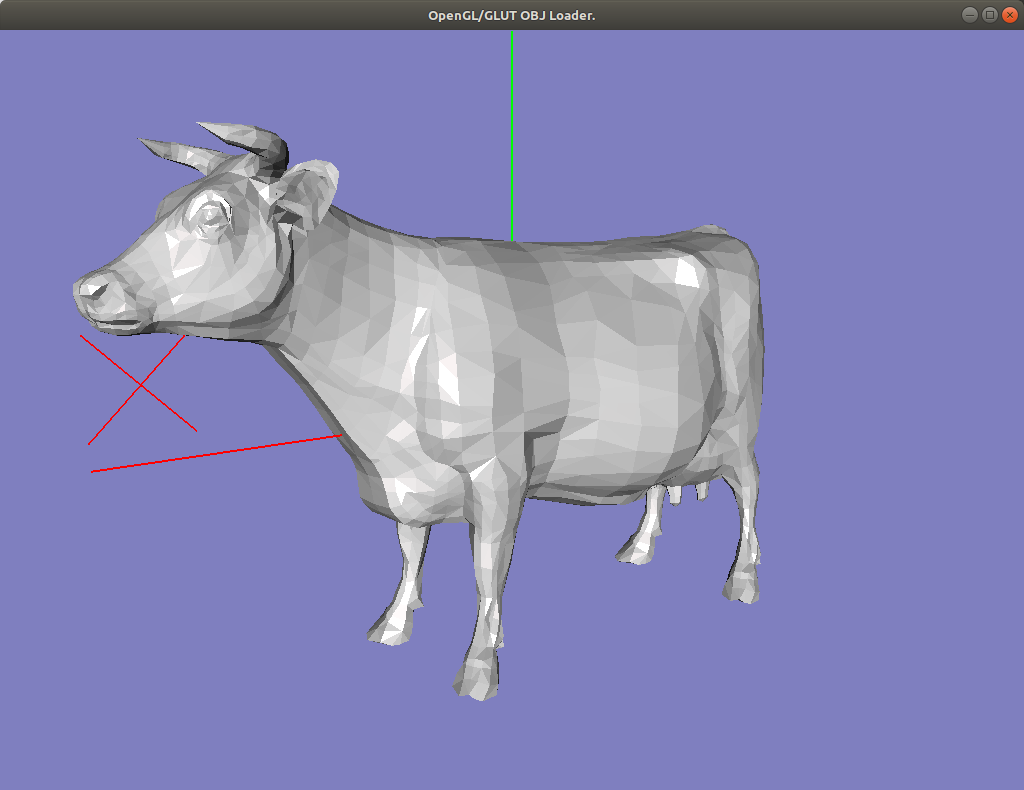
\includegraphics[width=.45\columnwidth]{cowflat.png}}
\subfigure[]{\includegraphics[width=.45\columnwidth]{cowsmooth.pdf}}
\caption{The same model rendered using a single face normal for each vertex (a) and its smoother version rendered using for each vertex an averaged normal of the surrounding faces (b).}
\label{fig:cowflatsmooth}
\end{center}
\end{figure}

%%%%%%%%%%%%%%%%%%%%%%%%%%%%%%%%%%%%%%%%%%%%%%%%%%%%%%%%%%%%%%%%%%%%%%%%%%%%%%%%%%%%%%%%%%%%%%%%%%%%%%%%%%%%%%%%%%%%%%%%%

\subsection{A more efficient rendering}

In the next step, we implement a more efficient way to render the model using the vertex array (see \sect{sec:arrays}). Moreover, we would like to have more pleasant visualization of the model, in which the surface of the model appears smoother and the single triangular faces are not visible. In order to do so, \opengl needs to have the normal for each vertex instead of a single normal for each face (hence common to each of the 3 vertices of the face). How can we compute a single normal to each vertex? Foe each vertex we can compute its normal as the average normal among all the faces it contributes to: \ie for each vertex, we can sum the normals of all its faces and then re-normalize the result.

\begin{enumerate}
    \item Complete the function \code{load()} in \coden{ObjModel.cpp}: whenever a new vertex is read set its normal to a zero vector. Then, whenever a face is read from the input file, compute the normal to the face and sum it to the normal of each vertex. At the end, when the file has been read, re-normalize all the normals.

    \item Complete the function \code{drawSmoothFaces()}: given the vertices, their normals and the mesh as input, draw the model using the vertex array in \opengl as explained in \sect{sec:arrays}.
\end{enumerate}

Once you have correctly implemented the function \coden{drawSmoothFaces()} you can turn this rendering on using the key \keystroke{S}. This will switch between the \coden{drawSmoothFaces()} and \code{drawFlatFaces()}. Also, the \keystroke{A} allows to switch from the \coden{GL\_SMOOTH} to \coden{GL\_FLAT} rendering.  Now you should be able to see a smoother rendering of the model when \coden{GL\_SMOOTH} and \coden{drawSmoothFaces()} are enabled.

\begin{figure}
\centering
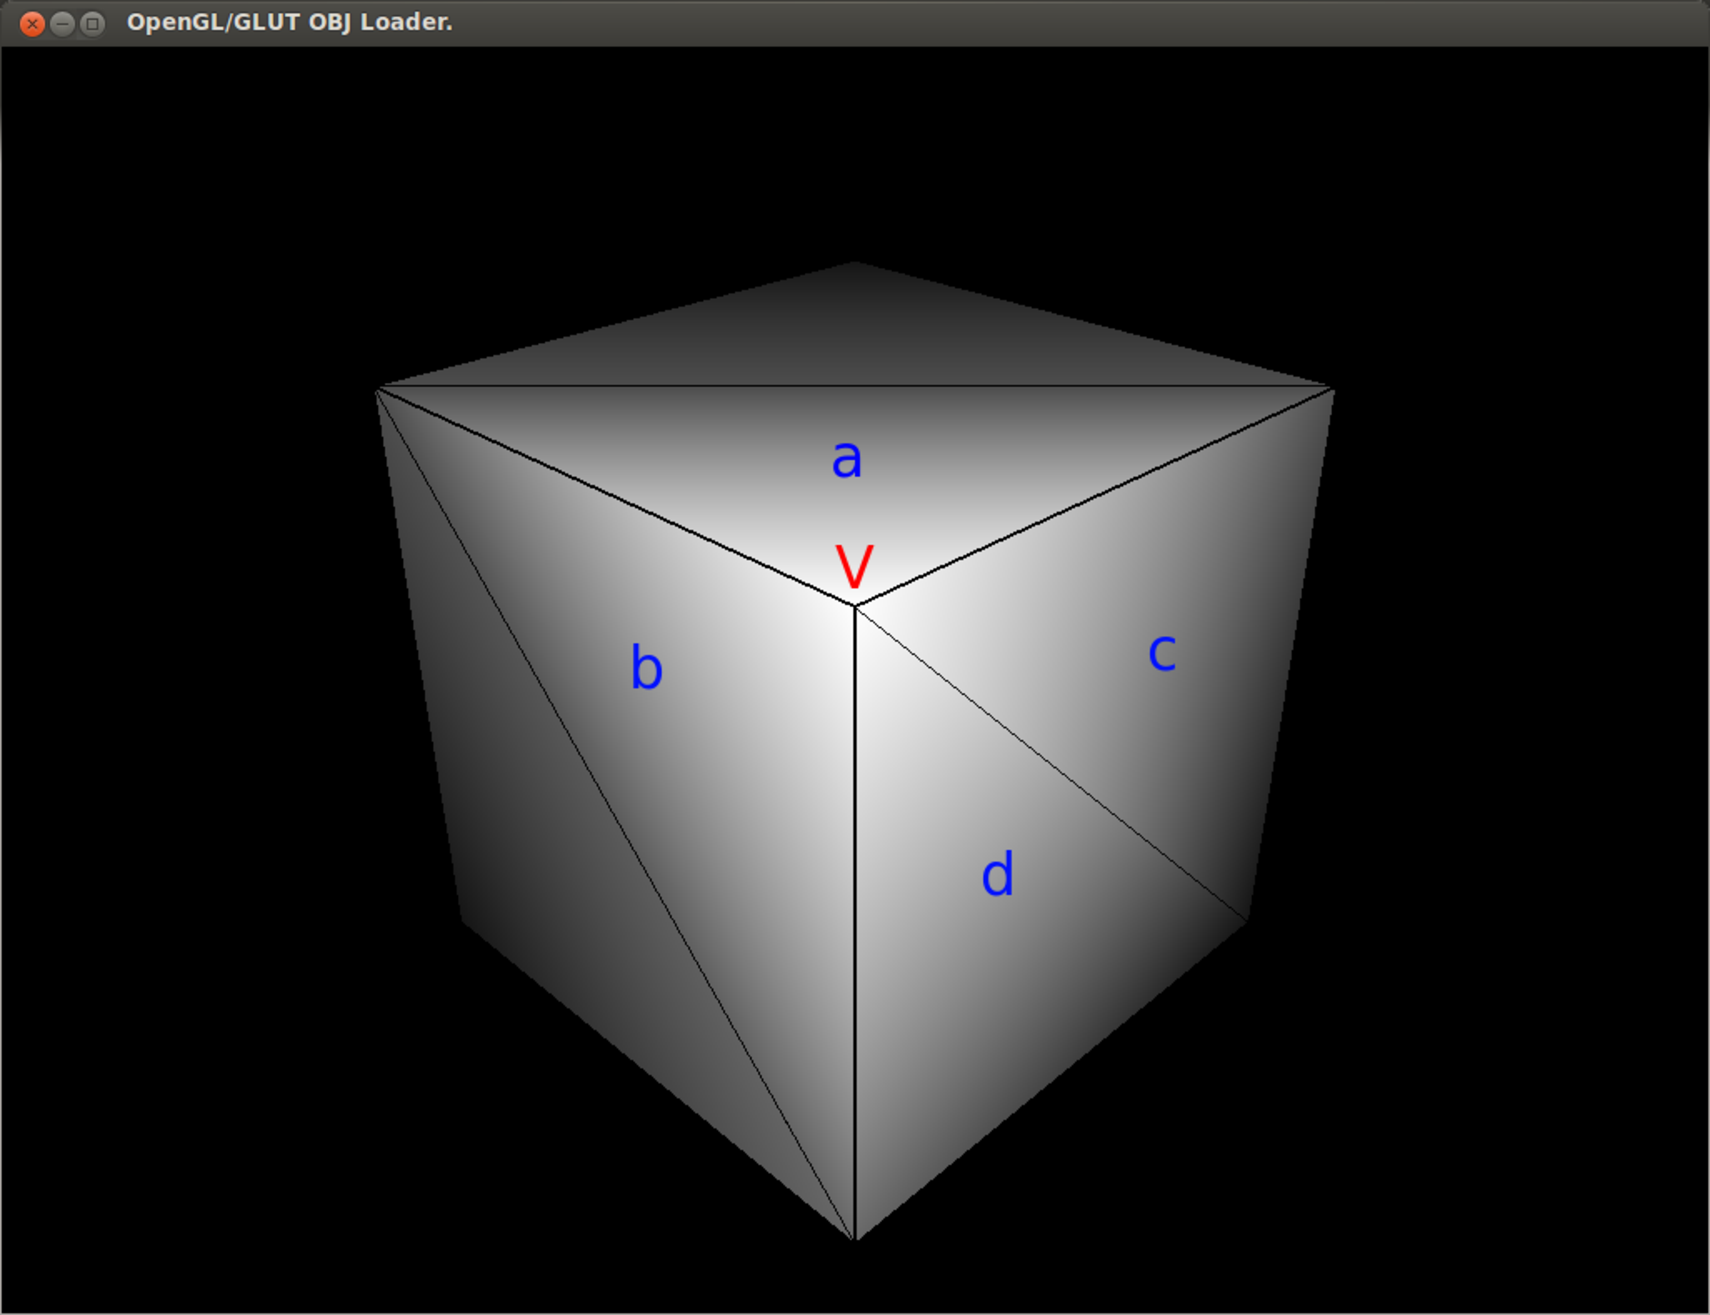
\includegraphics[width=.6\columnwidth]{cubenormal}
\caption{An example of the biased computation of the normals for the vertex $V$: it receives a contribution from the faces $a$ and $b$ and a double contribution with the same normal from the faces $c$ and $d$.}
\label{fig:cubenormal}
\end{figure}

On the other hand, this implementation is not quite satisfying for models like the cube (try it\ldots). The computed normals are indeed biased for some vertices because they may receive a double contribution from the two triangular faces of the same cube face and only one from the the triangular face of the other cube face (see \fig{fig:cubenormal}). In order to solve this issue we can weight the contribution of each normal with the angle formed at the vertex.

\begin{enumerate}
    \item Modify the way the normals are summed in function \code{load()}: for each vertex $V$ of the face, the normal of the face is weighted by the extent of the angle formed by the edges at the vertex $V$.
     \begin{itemize}
        \item To this end you can use the function \code{angleAtVertex()}: \\
{\smaller
\begin{cppcode}
/**
* Computes the angle at vertex baseV formed by the edges connecting it with the
* vertices v1 and v2 respectively, ie the baseV-v1 and baseV-v2 edges
* 
* @brief Computes the angle at vertex
* @param baseV the vertex at which to compute the angle
* @param v1 the other vertex of the first edge baseV-v1
* @param v2 the other vertex of the second edge baseV-v2
* @return the angle in radiants
*/
float angleAtVertex(const point3d& v1, const point3d& v2, const point3d& v3) const;
\end{cppcode}
}
        \end{itemize}
 \end{enumerate}   



%%%%%%%%%%%%%%%%%%%%%%%%%%%%%%%%%%%%%%%%%%%%%%%%%%%%%%%%%%%%%%%%%%%%%%%%%%%%%%%%%%%%%%%%%%%%%%%%%%%%%%%%%%%%%%%%%%%%%%%%%
\pagebreak

\section{Loop's subdivision}

The Loop subdivision scheme subdivides a triangular mesh surface by performing several iterations in which each (triangular) face is subdivided into 4 smaller ones. The algorithm starts with a set of points that are the vertices of triangles. Each iteration computes a new set of edge and vertex points that become the vertices of the new, smaller triangles. Specifically, a new edge point is computed for each edge and a new vertex point is computed for each vertex of the triangular mesh. If the original mesh has $E$ edges and $V$ vertices, the new mesh will have $E + V$ vertex points (and a number of edges that depends on the complexity of the original mesh).
The new points become the vertices of the new, finer mesh, and more iterations may be applied to refine the mesh as much as needed. 


\begin{figure} 
\centering  
\def\svgwidth{.6\columnwidth}
\includesvg{loopsubdiv}
\caption{An example of Loop subdivision algorithm applied to a triangular mesh. Each edge of the original mesh generates a new vertex $E_i$, and new smaller faces are formed connecting the new vertices $E_i$ and the original vertices $V_i$. \uline{Note that the vertices $E_i$ in general DO NOT lie on the edges, here they are placed on the edge just for readability of the figure.}}
\label{fig:loopsubdiv}  
\end{figure} 

Considering the simple mesh in \fig{fig:loopsubdiv} centered on the vertex $V$, the rule to generate the new vertices $E_i$ for each of the edge sharing $V$ is:

\begin{equation} \label{eq:ei}
E_i = \frac{3}{8} \left(V + V_i\right) + \frac{1}{8} \left(V_{i+1} + V_{i-1}\right),
\end{equation} 
whereas, for boundary edges such as $V_1$-$V_2$ (see \fig{fig:loopsubdiv}), the new vertex $A$ is the midpoint of the two extrema of the edge
\begin{equation} \label{eq:eib}
A = \frac{1}{2} \left(V + V_i\right) .
\end{equation} 

\noindent The original vertex $V$ is updated using the Loop's coefficients:
\begin{equation} \label{eq:vhat}
\hat{V} = \frac{5}{8} V  + \frac{3}{8} \frac{1}{n} \sum_i^n V_i.
\end{equation} 


\subsection{The Algorithm}

The algorithm to implement is relatively simple and it requires three main steps: (\emph{i}) generate the new vertices according to \eqref{eq:ei} and \eqref{eq:eib}, (\emph{ii}) update the original vertices according to \eqref{eq:vhat}, and finally (\emph{iii}) recompute the normals for all the vertices as you did in the \coden{load()} function.

The first part (\emph{i}) is maybe the trickiest part. Since we don't have a list of edges, we can consider each face and for each of its edges generate the new vertex. However, this requires to keep a record of every new generated vertex and the relevant edge that generated it, in order to avoid to replicate the vertices: \eg, considering the face $V$-$V_1$-$V_2$, we can generate the new vertices $E_1$, $E_2$ and $A$, but then, for the face $V$-$V_2$-$V_3$ we must be able to know that $E_2$ has been already created. For this reason, we will keep a database in which each entry has a unique key, the edge, and a value, the index of the corresponding generated vertex. For your convenience, the database structure is already implemented in the class \code{EdgeList} (see the doc in \sect{sec:edgelist}).

Finally, we can consider an edge as a pair of indices, one for each of the two vertex. Again, for your convenience, the corresponding data structure is already defined:


{\smaller
\begin{cppcode}
/**
 * An edge is defined as a pair of vertex indices 
 */
typedef std::pair<idxtype, idxtype> edge;

// exemples of usage
edge e(2, 3);           // create an edge e with vertex indices 2 and 3
idxtype v1 = e.first;   // get the first index (v1 == 2 in this case)
idxtype v2 = e.second;  // get the first index (v2 == 3 in this case)
\end{cppcode}
}


\subsection{Let's implement it}

In order to make things easier (I hope\ldots), the algorithm has been broken into two main functions. The function \code{loopSubdivision()} is the main one containing the 3 steps discussed above, and the one that is actually called to subdivide a mesh. The function \code{getNewVertex()} is a helper function that takes care of generating new vertices. 

\begin{enumerate}
    \item Complete the helper function \code{getNewVertex()} in \coden{ObjModel.cpp}: this function is used to generate a new vertex at a given edge during the subdivision process. It returns the index of vertex associated to the given edge. Check the complete list of its parameters in the source code. 
    \begin{itemize}
        \item In order to check whether an edge is a boundary egde you can use the function \code{isBoundaryEdge()}, which returns the indices of the two opposite vertices of the edge, or only one if the edge is a boundary edge (and only in this case it returns \coden{true}):

{\smaller[2]
\begin{cppcode}
/**
 * It checks if the edge e is a boundary edge in the list of triangle. It also 
 * return the indices of the two opposite vertices of the edge or only one of 
 * them if it is a boundary edge
 * 
 * @param[in] e the edge to check
 * @param[in] mesh the list of triangles
 * @param[out] oppVert1 the index of the first opposite vertices 
 * @param[out] oppVert2 the index of the second opposite vertices (if any)
 * @return true if the edge is a boundary edge
 */
bool isBoundaryEdge(const edge& e, const vector<face>& mesh, idxtype& oppVert1, idxtype& oppVert2 )
\end{cppcode}    
}

    \end{itemize}
    \item Complete the function \code{loopSubdivision()}: given a list of vertices and the relevant mesh as input, it returns a new list of vertices, their normals, and the new mesh corresponding to the output of one step of Loop's subdivision algorithm. 

    \begin{itemize}
        \item Again, we will work with the function parameters instead of the member of the class \coden{ObjModel}, so that the function is general and can be applied several times.

        \item The function implements the three main parts of the algorithm described above. They roughly corresponds to 3 main couples of \coden{for} loops:
        \begin{itemize}
            \item the first \coden{for} loop goes over all the faces to generate the new vertices and the new faces; it uses the database \code{newVertices}, an instance of \coden{EdgeList}, to keep track of the new vertices and the edges that originated them.

            \item The second \coden{for} loop updates the original vertices according to the Loop rule \eqref{eq:vhat}; again, since we don't have a neighbourhood relation for the vertices, we can update the vertices \uline{incrementally} going through each face: each vertex of a face is updated using \eqref{eq:vhat} with the other two vertices of the face. To this purpose, we can use an auxiliary vertex list \code{tmp} that cumulates the contribution from each face. For example, considering the vertex $V$ in \fig{fig:loopsubdiv}:
            \begin{itemize}
            	\item the first face $V$-$V_1$-$V_2$ updates $V$ using $V_1$ and $V_2$, the second face $V$-$V_2$-$V_3$ using $V_2$ and $V_3$, and so on.
            	\item Be careful though, as this way each $V_i$ is contributing twice, hence a small change in the coefficients of \eqref{eq:vhat} is required\ldots
            	\item We are not quite finished yet, as we also need to divide the final cumulated sums by the number of faces in which the vertex has been seen (this corresponds to the $\frac{1}{n}$ in \eqref{eq:vhat}). For this, we can keep another list of integer \code{occurrences} that is updated every time a vertex is updated\footnote{As you can probably note, this is actually a simplification, it will only works with manifold meshes without boundaries. If you want to implement it correctly you have to built a proper data structure to have the neighbourhood relation of vertices\ldots}.
             \end{itemize}

            \item The third and final \coden{for} loop updates the normals associated to each vertex of the new mesh, in a similar way as you already did for the \coden{load()} function.
        \end{itemize}
    \end{itemize}
\end{enumerate}

Once you are done implementing the algorithm you can switch between the original model and its subdivide version using the key \keystroke{H}. Moreover, you can use the keys \keystroke{1} \ldots \keystroke{4} to apply $n=1\div4$ iteration of the Loop algorithm. It may be wise not to apply more than 2 subdivision iterations to large meshes (it may take a while\ldots).

You can try the program with the different 3D models that you can find in \code{data} folder. Avoid to apply too many subdivision steps for large meshes. You should note something \emph bizarre happening when subdividing some of the models, \eg the cow or the teapot. In order to find what could cause this problem you can try to look at the normals of the vertices  where the problem occurs (key \keystroke{N}): try to compare the affected vertices and the normal(s) on the original mesh and on the subdivide model, you should note something strange going on on those vertices... Any clue?


%%%%%%%%%%%%%%%%%%%%%%%%%%%%%%%%%%%%%%%%%%%%%%%%%%%%%%%%%%%%%%%%%%%%%%%%%%%%%%%%%%%%%%%%%%%%%%%%%%%%
\appendix
\section{The EdgeList class}
\label{sec:edgelist}

{\smaller
\begin{cppcode}
/**
 * A helper class containing the indices of the new vertices added with the subdivision
 * coupled with the edge that has generated them. More specifically, it is a list in which
 * each entry has a key (ie an identifier) and a value: the key is the edge that
 * generate the vertex, the value is the index of the new vertex.
 * The key (ie the edge) is unique, ie an edge cannot generate more than one vertex. The
 * edge is a pair of vertex indices, two edges are the same if they contain the 
 * same pair of vertices, no matter their order, ie
 * edge(v1, v2) == edge(v2, v1)
 * 
 * @see edge
 */
class EdgeList
{
public:

    /**
     * Add the edge and the index of the new vertex generated on it
     * @param[in] e the edge
     * @param[in] idx the index of the new vertex generated on the edge
     */
    void add( const edge& e, const idxtype& idx );

    /**
     * Return true if the edge is in the map
     * @param[in] e the edge to search for
     * @return true if the edge is in the map
     */
    bool contains( const edge& e ) const;

    /**
     * Get the vertex index associated to the edge
     * @param e the edge
     * @return the index
     */
    idxtype getIndex( const edge& e );
...
}
\end{cppcode}
}

\section{The full key mapping}
\label{sec:keymapping}
Key mapping for the viewer:
\begin{itemize}
    \item \keystroke{W} enable/disable wireframe
    \item \keystroke{A} enable/disable \coden{GL\_SMOOTH} rendering (\ie shading)
    \item \keystroke{S} enable/disable index rendering
    \item \keystroke{D} enable/disable solid rendering of the mesh (\ie no face color)
    \item \keystroke{H} switch between the original model and its subdivided version
    \item \keystroke{N} show/hide vertex normals
    \item \keystroke{1}\ldots\keystroke{4} apply 1 \ldots 4 steps of subdivision
    \item You can move around the 3D model (once displayed) with the usual arrow keys and use \keystroke{PgUp}, \keystroke{PgDn} to zoom in/out.
\end{itemize}
\end{document}
